\section{Scale factors for Primakoff, nuclear coherent, and nuclear incoherent cross sections  \label{sec:SigmaScaling}}
Fig.~\ref{fig:leaddndt} shows $^{208}$Pb data from the PrimEx experiment \cite{Larin:2010kq}.   NPP will run on the same target and the same approximate incident beam energy, $\approx 6$ GeV, as PrimEx.   Using known analytical forms for the processes shown in the figure, known photo-nuclear cross sections, and estimates for nuclear attenuation from the PrimEx $^{208}$Pb analysis, we estimate numerical factors for scaling the Primakoff, nuclear coherent and nuclear incoherent total cross sections seen in PrimEx to the conditions for NPP. 
    

 \subsection{Scale factor for the Primakoff cross section}
The standard equation for Primakoff $\pi^0$ production is given by: 

$$ { d^2 \sigma_{PrimEx} \over d \Omega } = \Gamma_{\pi^0 \rightarrow \gamma \gamma} { 8 \alpha Z^2 \over M^3_{\pi} }
{ \beta^3 E_\gamma^4 \over Q^4 } F^2_{EM}(Q^2) sin^2 \theta   $$ 
where $\Gamma_{\pi^0 \rightarrow \gamma \gamma} = 7.7$ eV is the $\pi^0$ radiative width.  The cross section for Primakoff $\pi \pi$ production with $P_{\gamma}=0$ is given by: 
$$ {d^2 \sigma_{NPP} \over d \Omega_{\pi \pi} dM_{\pi \pi} } = {2 \alpha Z^2 \over \pi^2} 
{E_\gamma^4 \beta^2 \over M_{\pi \pi} } {sin^2 \theta \over Q^4 } F^2_{EM}(Q^2) 
 \sigma( \gamma \gamma \rightarrow \pi \pi) $$
The above equation can be reorganized so that it has a structure similar to the standard Primakoff equation: 
$$ {d^2 \sigma_{NPP} \over d \Omega_{\pi \pi} } \approx
\Big[ {1 \over 4 \pi^2 }  {M^2_{\pi \pi} \over \beta }  \sigma( \gamma \gamma \rightarrow \pi \pi) \Delta M_{\pi \pi} \Big]  { 8 \alpha Z^2 \over M^3_{\pi \pi} }
{ \beta^3 E_\gamma^4 \over Q^4 } F^2_{EM}(Q^2) sin^2 \theta  $$
$$ {d^2 \sigma_{NPP} \over d \Omega_{\pi \pi} } \approx
\Gamma_{\pi^0 \pi^0 \rightarrow \gamma \gamma}  { 8 \alpha Z^2 \over M^3_{\pi \pi} }
{ \beta^3 E_\gamma^4 \over Q^4 } F^2_{EM}(Q^2) sin^2 \theta  $$
where  $\Gamma_{\pi^0 \pi^0 \rightarrow \gamma \gamma}$ is the effective radiative width for $\pi^0 \pi^0 \rightarrow \gamma \gamma$, 
$$ \Gamma_{\pi^0 \pi^0 \rightarrow \gamma \gamma} =\Big[ {1 \over 4 \pi^2 }  {M^2_{\pi \pi} \over \beta }  \sigma( \gamma \gamma \rightarrow \pi \pi) \Delta M_{\pi \pi} \Big] $$
Taking $M_{\pi \pi} \approx 0.4$ GeV, $\Delta M_{\pi \pi}\approx 0.4$ GeV, and $\sigma ( \gamma \gamma \rightarrow \pi^0 \pi^0) \approx 10$ nb gives, 
$$\Gamma_{\pi^0 \pi^0 \rightarrow \gamma \gamma} \approx 42\ eV$$

The angular dependence of the Primakoff differential cross section for single and double-pion production is given by,
$$ {d\sigma \over d \Omega} \sim {sin^2 \theta \over Q^4}|F(Q^2)|^2$$
It can be shown (see notes from R. Miskimen) that the peak of the Primakoff differential cross section is at the angle,
$$ \theta_{max}={s \over 2 E^2_\gamma}$$
where s is the invariant mass of the $\pi$ or $\pi \pi$ system.  The factor $|F(Q^2)|^2$ has a negligible effect on the position of the peak. 

The total cross section is given by the integral

$$ \sigma \sim \int^{C\theta_{max}}_0 {sin^2 \theta \over Q^4}|F(Q^2)|^2 2 \pi sin \theta d\theta$$
where \it C \rm is a dimensionless scale factor. Working in the small angle limit the total cross section is,
$$\sigma \sim 2\pi \int^{C\theta_{max}}_0 
{\theta^3 \over \left( {s^2 \over 4E^2_\gamma}+ E^2_\gamma \theta^2  \right)^2} 
\Big[ 1-{1 \over 6}<r^2>_{charge}\left( {s^2 \over 4E^2_\gamma}+ E^2_\gamma \theta^2  \right)\Big]^2
d \theta$$
$$\sigma \sim 2\pi \int^{C\theta_{max}}_0 
{\theta^3 \over \left( {s^2 \over 4E^2_\gamma}+ E^2_\gamma \theta^2  \right)^2} 
\Big[ 1-{1 \over 3}<r^2>_{charge}\left( {s^2 \over 4E^2_\gamma}+ E^2_\gamma \theta^2  \right)\Big]
d \theta$$
Making a change of variable and performing the integration leads to the result, 
$$ \sigma \sim {\pi \over E^4_\gamma}
\left[ \Big( ln(1+C^2)-{C^2 \over 1+C^2}  \Big)
- {1 \over 12}<r^2>_{charge}{s^2 \over E^2_\gamma}
\Big(C^2-ln(1+C^2 \Big) \right]$$
For C=4 the term on the left within the brackets sums to +1.89, and the term on the right ( proportional to $<r^2>$) sums to -0.008 (-.61) for the $\pi (\pi \pi)$ final state.  Then the ratio of integrals for double pion to single pion Primakoff production is approximately $I_{\pi\pi} / I_{\pi} \approx 0.68$
The total cross section is approximately proportional to $1/E^4_\gamma$, nearly canceling the E$^4_\gamma$ factor in the Primakoff equations, and leading to the result that the total cross section is approximately independent of incident photon energy.   


Our final result for the ratio of Primakoff cross sections $\sigma_{\pi^0 \pi^0}$ to $ \sigma_{\pi^0}$ is given by, 
$$  \sigma_{\pi^0 \pi^0}   \Big/ \sigma_{ \pi^0}   
\approx 
\Big(\Gamma_{\pi^0 \pi^0 \rightarrow \gamma \gamma}
\Big/ \Gamma_{\gamma \gamma} \Big)
\times \Big( M_\pi \Big/ 
M_{\pi \pi}\Big)^3\times \Big( I_{\pi \pi} \Big/ I_\pi \Big)
\approx 0.14$$



 \subsection{Scale factor for the nuclear coherent cross section}

The nuclear coherent cross section for  $\pi^0$ photo-production is given by: 

$$ {d\sigma_{\gamma A \rightarrow A  \pi^0 } \over dt } \approx \eta A^2 { d\sigma_{\gamma N \rightarrow N \pi^0 } \over dt }sin^2 \theta F^2(t) $$
where $\eta$ is the nuclear absorption factor for $\pi^0$ production, A is the atomic mass number, $d\sigma_{\gamma N \rightarrow N\pi^0 } / dt$ is the $\pi^0$ photo-production cross section on the nucleon, and $F(t)$ is the nuclear matter formfactor.  The nuclear coherent cross section for  $\pi^0 \pi^0$ photo-production has a similar form: 

$$ {d\sigma_{\gamma A \rightarrow A  \pi^0 \pi^0} \over dt } \approx  \eta^2 A^2 { d^2 \sigma_{\gamma N \rightarrow N \pi^0 \pi^0} \over dt dM_{\pi \pi}}\Delta M_{\pi \pi} sin^2 \theta F^2(t) $$
where $d^2\sigma_{\gamma \rightarrow N\pi^0 \pi^0} / dt dM_{\pi \pi}$ is the $\pi^0 \pi^0$ photo-production cross section on the nucleon.
  In the near threshold region the dominant channel for $\pi^0 \pi^0$ is through f$_0(500)$ photo-production.    Cross sections for f$_0(500)$   have been measured in 
  $\gamma p \rightarrow \pi^+ \pi^-$ at 3.6-3.8 GeV \cite{Battaglieri:2009aa}.   The s-wave t and $M_{\pi^+ \pi^-}$ distributions are shown in Fig. \ref{f0_500}, the former at M$_{\pi \pi}=0.4$ GeV, and the latter at $t=0.5 GeV^2$.  Note that  
  $d\sigma^2 / dt dM_{\pi^+ \pi^-}$ is relatively flat versus M$_{\pi \pi}$ in the threshold region. The relevant cross section for this analysis is $d\sigma^2 / dt dM_{\pi^+ \pi^-}|_{ t = 0} \approx 1.0 \mu b/GeV^3$  multiplied by an isospin factor of 1/2 to account for the f$_0(500)$ branching fraction to $\pi^0 \pi^0$, giving $d \sigma_{\gamma N \rightarrow N \pi^0 \pi^0} / dt dM_{\pi \pi} \approx 0.5 \mu b / GeV^2 $. The cross section for  $\gamma p \rightarrow  p \pi^0$ at 6 GeV has been measured at SLAC \cite{Anderson:1971}, with cross sections shown in Fig. \ref{SLAC};   $d\sigma / dt|_{t=0} \approx 1.5 \mu b/GeV^2$ .   Estimates from the PrimEX $^{208}$Pb analysis give $\eta \approx 0.55$.  
  
  Assuming an exponential behavior for the differential cross section on the nucleon, 
  $$ {d\sigma_{\gamma N \rightarrow N X} \over dt} = \sigma_0 e^{-kt}$$
  the coherent angular distribution is given by
  $$ { d\sigma_{coherent} \over d\Omega} = \sigma_0 sin^2 \theta |F(t)|^2 e^{-kt} {dt \over d\Omega}$$ 
  For CPP and NPP we have, 
  $$ {2k \over <r^2>_{matter}}<<1 $$
  and 
  $${1 \over 6}<r^2>_{matter} {s^2 \over 4E^2_\gamma}<<1$$
   To leading order in $\theta^2$ the peak coherent cross section is at angle 
$$ \theta_{max}={1 \over E_\gamma}\sqrt{ 2 
 \over <r^2>_{matter} } $$
 . 
 
  The total cross section is given by, 
  $$ \sigma_{coherent} \sim \sigma_0 \int^{C\theta_{max}}_0 sin^2 \theta |F(t)|^2 e^{-kt} {dt \over d\Omega} 2\pi sin\theta d\theta$$ 
  where C is a dimensionless scale parameter. Working in the small angle approximation
  and using the condition, 
 $$k\big( {s^2 \over 4 E^2_\gamma} \big) <<1$$
 we can reduce the total cross section  to this form, 
  $$ \sigma_{coherent} \sim {8\sigma_0 \over <r^2_{charge}>^2E^2_\gamma}
  \int^C_0 y^3 \Big[1- {1 \over 3} y^2 \Big]^2 dy  $$ 
  Since the integral depends only on C, the integral cancels out in taking the ratio
  $\sigma_{\gamma A \rightarrow A \pi^0 \pi^0}   \Big/  \sigma_{\gamma A \rightarrow A \pi^0} $. 
  
  Here we give our final result for the ratio of  $\pi^0 \pi^0$ to $\pi^0$  coherent cross sections:

$$  \sigma_{\gamma A \rightarrow A \pi^0 \pi^0}   \Big/  \sigma_{\gamma A \rightarrow A \pi^0}  \approx \eta 
 {d^2\sigma_{\gamma N \rightarrow N \pi^0 \pi^0} \over dt dM_{\pi \pi} } \Delta M_{\pi \pi} \Big/ { d\sigma_{\gamma N \rightarrow N \pi^0} \over dt} \approx 0.07 $$

\subsection{Scale factor for the nuclear incoherent cross section}

The incoherent cross section for  $\pi^0$ photo-production is given by: 

$$ {d\sigma_{\gamma A \rightarrow   \pi^0 } \over dt } \approx \eta A \Big(1 -G(t) \Big){ d\sigma_{\gamma N \rightarrow N \pi^0 } \over dt } $$
where G(t) is a Pauli suppression factor, with G(0)=1 and $G(t)\rightarrow 0$ for $t> k_F$, where $k_F$ is the nuclear Fermi momentum, $k_F\approx 260$ MeV/c. The incoherent cross section for  $\pi^0 \pi^0$ photo-production has a similar form: 
$$ {d\sigma_{\gamma A \rightarrow   \pi^0 \pi^0 } \over dt } \approx \eta^2 A \Big(1 -G(t) \Big){ d^2\sigma_{\gamma N \rightarrow N \pi^0 \pi^0 } \over dt dM_{\pi \pi}} \Delta M_{\pi \pi} $$
The photo-production cross sections on the nuclon are identical to those used in the estimation of the coherent cross section.   

The total cross section is given by, 
$$\sigma \sim \sigma_0 \int^{C E^2_\gamma \theta^2_{max}}_{s^2/4E^2_\gamma} \Big( 1 - G(t) \Big) e^{-kt} dt  $$
where we integrate up to a multiple of $E_\gamma^2 \theta_{max}^2$, where $\theta_{max}$  is the angle of the peak coherent cross section, and $s^2/4E^2_\gamma$ is the minimum t in the reaction.  
Because $s^2/4E^2_\gamma << k^2_F$ and $1-G(s^2/4E^2_\gamma) \approx 0$, the lower limit on the integral can be replaced with zero, 
$$\sigma \sim \int^{CE^2_\gamma \theta^2_{max}}_0 \Big( 1 - G(t) \Big) e^{-kt}  dt $$
For $\pi$ or $\pi \pi$ photo-production 
$$ C  E^2_\gamma \theta^2_{max} k \approx C  { 2 \over <r^2>_{matter} } k << 1 $$
provided that $C \le 5$. In this case we can neglect the exponential in the integral, 
$$\sigma \sim \int^{C E^2_\gamma \theta^2_{max}}_0 \Big( 1 - G(t) \Big) dt $$
Since the integral depends only on the upper integration limit,   the integral  cancels out in taking the ratio $ \sigma_{\gamma A \rightarrow  \pi^0 \pi^0}  \Big/ \sigma_{\gamma A \rightarrow  \pi^0} $. 
Our final result for the ratio of  $\pi^0 \pi^0$ to $\pi^0$ incoherent cross sections is given by: 

$$  \sigma_{\gamma A \rightarrow  \pi^0 \pi^0}  \Big/ \sigma_{\gamma A \rightarrow  \pi^0}  \approx \eta 
 {d^2\sigma_{\gamma N \rightarrow N \pi^0 \pi^0} \over dt dM_{\pi \pi} }  \Delta M_{\pi \pi}\Big/ { d\sigma_{\gamma N \rightarrow N \pi^0} \over dt} \approx 0.07 $$

\subsection{Summary}
NPP will take data on the same target, $^{208}$Pb, and the same approximate incident beam energy, $\approx 6$ GeV, as PrimEx. Using known analytical expressions for the Primakoff, nuclear coherent, and nuclear incoherent cross sections, known photo-nuclear cross sections, and estimates for nuclear attenuation from the PrimEx $^{208}$Pb analysis, numerical factors are calculated to scale the total cross sections seen in PrimEx to the 
conditions for NPP.  Assuming $M_{\pi^0 \pi^0} \approx 0.4$ GeV, and a width  $\Delta M_{\pi^0 \pi^0} \approx 0.4$ GeV, the scale factors for Primakoff, nuclear coherent, and nuclear incoherent total cross sections are approximately $\times 0.14$, $\times 0.07$, and $\times 0.07$, respectively. 

\begin{figure}
\centering
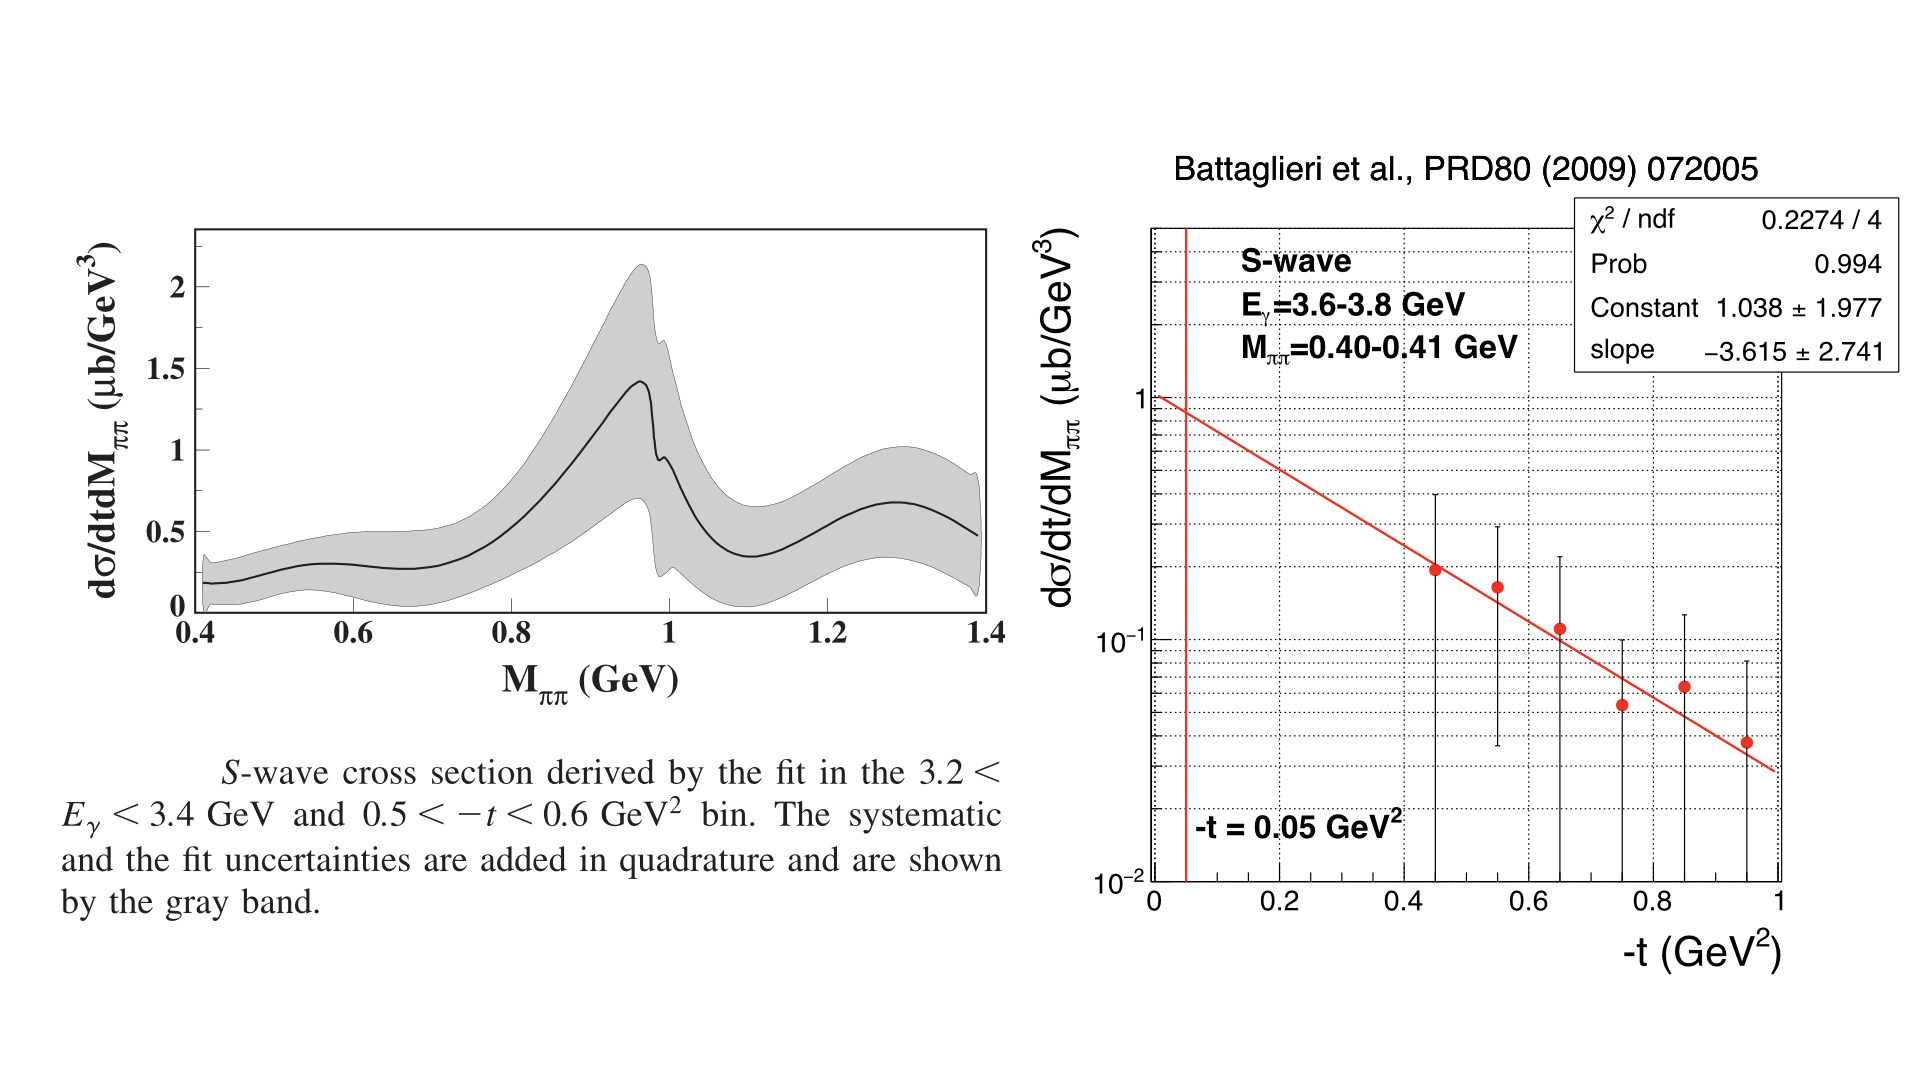
\includegraphics[width=6in]{figures/f0_500.png}
\caption{CLAS data for s-wave $\pi^+ \pi^-$ photoproduction on the proton at $3.2 < E_\gamma < 3.4$ GeV \cite{Battaglieri:2009aa}. }
\label{f0_500}
\end{figure}

\begin{figure}
\centering
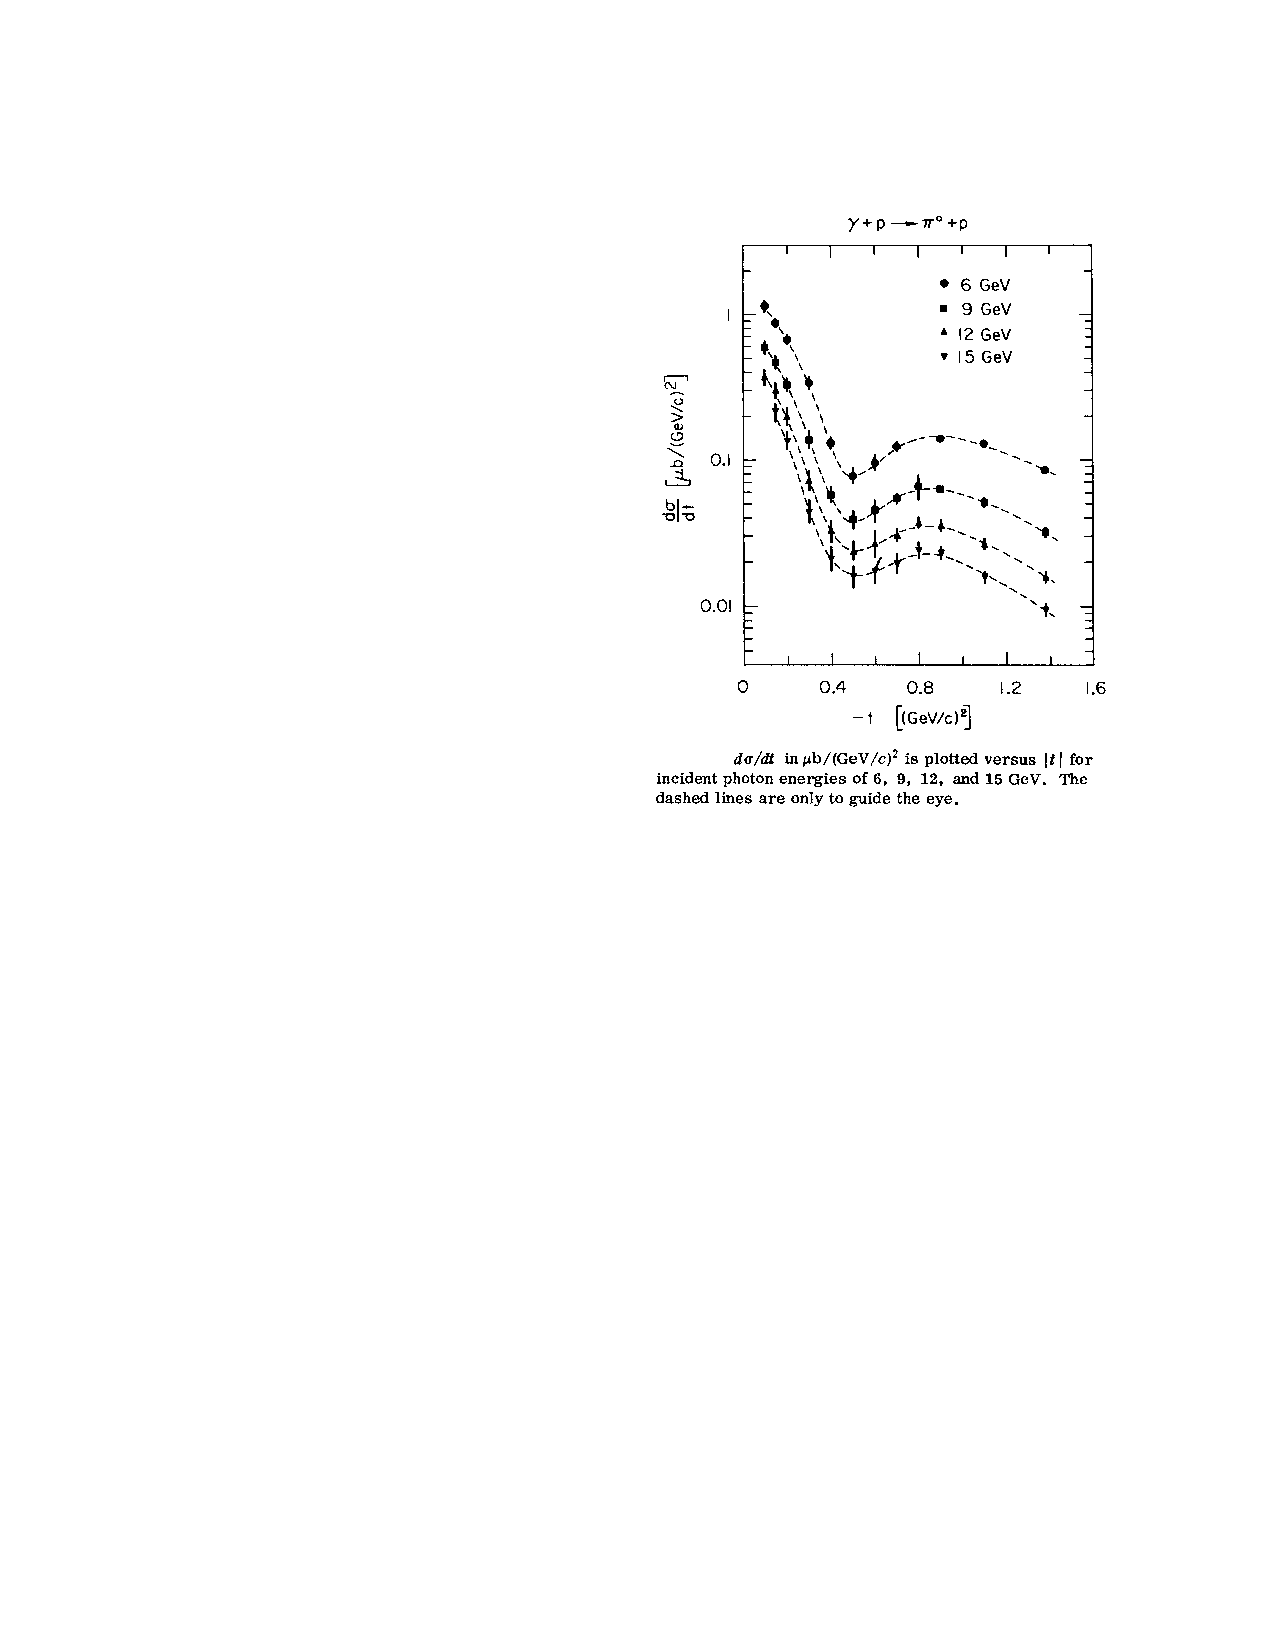
\includegraphics[width=4in]{figures/SLAC_data.pdf}
\caption{SLAC data for $\pi^0$ photo-production on the proton \cite{Anderson:1971}.}
\label{SLAC}
\end{figure}